\subsubsection{26.01.15}
\begin{enumerate}
	
	\item Время начала и окончания собрания: 17:15 - 22:00.
	
	\item Цели собрания: 
	\begin{enumerate}
		
		
		\item Подключить сервопривод, отвечающий за захват корзин.
		
		\item Продолжить тренировки по управлению роботом.
		
        \item Установить защиту от столкновений на NXT-блок и Samantha-модуль.
		
	\end{enumerate}

	\item Проделанная работа:
	\begin{enumerate}
		
		\item Сервопривод был подключен и прописан в программах автономного и управляемого периодов.
		
		\item Защита на NXT-блок и Samantha-модуль была установлена.
		\begin{figure}[H]
		  \begin{minipage}[h]{0.47\linewidth}
			\center{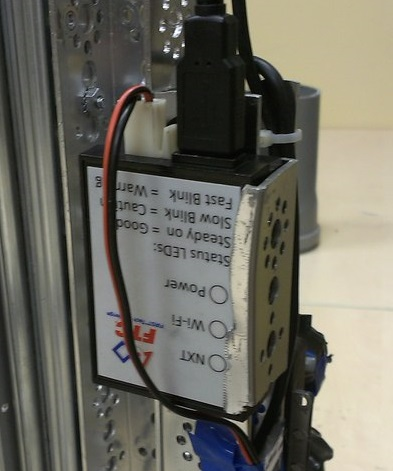
\includegraphics[scale=0.3]{days/26.01.15/images/01}}
			\caption{Защита Samantha-модуля}
		  \end{minipage}
		  \hfill
		  \begin{minipage}[h]{0.6\linewidth}
			\center{
\includegraphics[scale=0.5]{days/26.01.15/images/02}}
			\caption{Защита NXT-блока}
		  \end{minipage}
	    \end{figure}
		
        \item Сегодня к нам в голову пришла идея усовершенствовать механизм захвата мячей. Сервопривод свободного вращения, приводящий в движение ось с лопатками, вращается слишком медленно и с маленьким усилием, поэтому мы решили заменить его на пару моторов LEGO NXT 2.0, расположенных по обе стороны от оси. Было реализовано два переходника с вала LEGO-мотора на ось из набора TETRIX, моторы были закреплены на роботе и защищены щитками из оцинкованной стали.
        \begin{figure}[H]
	  	  \begin{minipage}[h]{0.47\linewidth}
	  	    \center{
\includegraphics[scale=0.2]{days/26.01.15/images/03}}
	  	  \end{minipage}
	  	  \hfill
	  	  \begin{minipage}[h]{0.24\linewidth}
	  		\center{
\includegraphics[scale=0.2]{days/26.01.15/images/04}}
	  	  \end{minipage}
	  	  \hfill
	  	  \begin{minipage}[h]{0.24\linewidth}
	  	  	\center{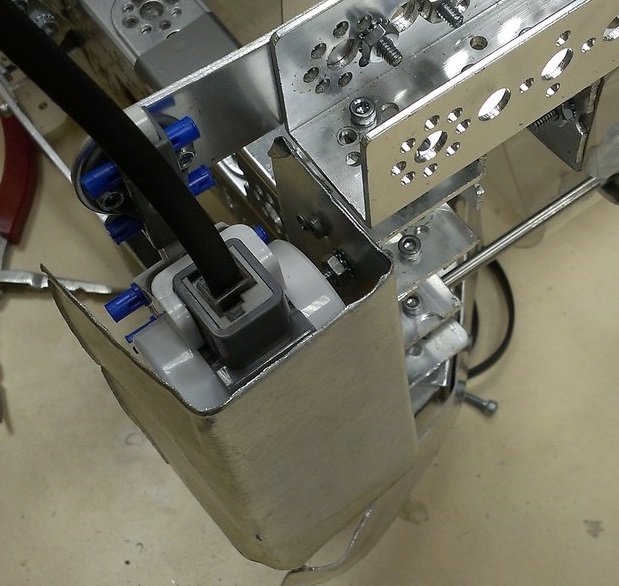
\includegraphics[scale=0.2]{days/26.01.15/images/05}}
	  	  \end{minipage}
	  	  \caption{Модифицированный механизм захвата мячей}
	   \end{figure}
	   
	   \item После того, как моторы были подключены и программа изменена под них, мы провели полевые испытания робота. Результат превзошел ожидания: захват вращался в три раза быстрее прежнего и был в несколько раз мощнее. Мячи захватывались очень быстро и так разгонялись, что вылетали в ковш. Благодаря этому они не застревали между осью захвата и горизонтальной балкой, как раньше. С таким захватом нам будет гораздо проще набирать мячи и дело пойдет быстрее.
	   
	   \item 28-29 января мы полетим в Пермь на соревнования, поэтому нам необходимо на следующем занятии (завтра) усердно потренироваться, а затем упаковать робота для поездки.

	\end{enumerate}
	
	\item Итоги собрания:
	\begin{enumerate}
		
		\item Сервопривод дополнительного захвата мячей подключен.
		
		\item NXT-блок и Samantha-модуль защищены от столкновений.
		
        \item Механизм захвата мячей модифицирован и испытан. Результат очень положительный.
		
	\end{enumerate}
	
	\item Задачи для последующих собраний:
	\begin{enumerate}
		
		\item Продолжить тренировки.
		
		\item Упаковать робота для поездки на соревнования в Пермь.
			
	\end{enumerate}
\end{enumerate}
\fillpage
